\newpage
\section{Tainting Dependencies}
\label{sect:trans:taintingDependencies}

\begin{itemize}
  \item \textbf{\LARGE TODO:} det er en newpage p\aa~denne siden
  \item INTRO for teh wind
  \item har vokst ut av MarkXRemove
  \item Tainting dependencies (TD)
  \item og mer text
\end{itemize}

\subsection{Inference Rule Language Explanation}
\label{sect:trans:TD:langExpl}
\underline{\textbf{\LARGE TODO:}} Skal jeg bruke greske bokstaver i stedet for tekstlig marsgreie n\aa r jeg
skriver regler?

During this chapter we will present some inference rules. In this section we will explain the various
typographical representations.

\begin{table}[h]
\centering
\begin{tabular}{l|l}

  $\longmapsto$  			& Translates into \\
  $\vartheta$ 				& A set of iterator dependencies \\
  \textsf{sans serif} 		& MQL expressions \\
  \texttt{monospaced} 		& XQuery expressions \\
  $e,\ldots,e_{n}$			& Generic expressions \\
  $\chi,\ldots,\chi_{n}$	& Generic variable names \\
  $I_{\chi}$				& The iterator expression which declares $\chi$ \\
  \textbf{bold} 			& Operations done during the generation of the algebra \\
  \textbf{r(}$e$\textbf{)} 	& Returns the relational algebraic representation of $e$   \\
  \textbf{t(}\textbf{r(}$e$\textbf{)}\textbf{,}$\vartheta'$\textbf{)} & Returns \textbf{r(}$e$\textbf{)} tainted
  with the dependencies $\vartheta'$ \\
  $\Delta$ 					&  The default context \\ 
  $\Lambda$ 				& The logical/boolean context \\
  
\end{tabular}
\caption{Explanation of inference rule symbols}
\label{tab:trans:td:langExpl}
\end{table}

Inference rules are generally in this format:
\begin{equation*}
\frac{\mbox{\textbf{cxt}}\vdash cond}{e}\longmapsto \mbox{\textbf{r(}}e\mbox{\textbf{)}}
\end{equation*}

This should be read as: in the context of \textbf{cxt}, if condition $cond$ is satisfied, the XQuery expression
$e$ will be translated into \textbf{r(}$e$\textbf{)}.

The translator is in the logical context, $\Lambda$, if the AST node it is currently visiting is a successor of a
boolean operator or within the condition part of an \texttt{if..then..else} expression. In all other cases the
translator is in the default context, $\Delta$. If no context is mentioned in the inference rules the default
context is assumed.

Often MQL operator trees are depicted like this:
\begin{center}
\begin{tabular}{l}
\textsf{operator1(\ldots,l.field, r.field\ldots; } \\ \quad
\textsf{operator2(\ldots);} \\ \quad
\textsf{operator3(\ldots))}
\end{tabular}
\end{center}

This is to be interpreted as \textsf{operator2} is the left child of \textsf{operator1} and \textsf{operator3} is
the right child. Mars does not allow attribute names to contain punctuation marks or allow two attributes with the
same name within one relation. An operator combining two relations will therefore have renaming functionality. A
typical projection list of such an operator combining two relations which both contain the attribute $field$ would
look something like: \textsf{\ldots rfield=right.field, lfield=left.field\ldots}. To make the inference rules
easier to read, this step has been dropped. The rules assume that the equal named fields will automaticly be given
a prefix \textsf{l.} (left) or \textsf{r.} (right) depending on which child the attribute stems from.

\section{Basics}
\label{sect:trans:TD:basics}
The method assumes left-to-right traversal of the assymetric syntax tree. In most cases the traversal is
postorder, meaning a subtree can be evaluated independently from its ancestors -- the exception being the logical
context set by boolean operators. The relational algebra will thus be generated bottom-up. In addition to the
evaluated subtree, a node must be able to inform its parent node about its variable dependencies ($\vartheta$),
which we will discuss later.

One XQuery sequence is represented as one relation and one XQuery item is represented as one tuple. This is sound,
as all XQuery items are sequences, and all sequences are one-dimensional (section
\ref{sect:theory:xquery:basics}). As we mentioned in section \ref{sect:trans:MarkXRemove}, the MarkXRemove method
did actually not consider the ordering of items in sequences at all. In Tainting Dependencies, however, we have
introduced an attribute $index$ holding the intra sequence number of the item. Consider the XQuery sequence
\texttt{('a','b',}$\ldots$\texttt{,'z')}. With this attribute, the relational representation will be as follwing:

\begin{center}
\begin{tabular}{|c|c|} \hline
$index$ & $value$ \\\hline
1		& \texttt{'a'} \\\hline
2		& \texttt{'b'} \\\hline
$\ldots$& $\ldots$ \\\hline
$n$		& \texttt{'z'} \\\hline
\end{tabular}
\end{center}


As can be seen, the item value is stored in the $value$ attribute. For the course of this chapter we will, for the
sake of simplicity, treat $value$ as a polymorphic type attribute. This simplification has minimal consequences
for the method and the way XQuery expressions are translated. XQuery types and relational representation of such
will is handled in section \ref{sect:disc:typeSystem}.

Also for simplicity, the $index$, $documentId$, $pos$ and $scope$ attributes have sometimes been left out of the
fields specified in \textsf{project} operators. If the \textsf{project} operator is applied to the result of a
join or cartesian product, these fields will follow the $value$ attribute if nothing else is specified. That is, if
$r.value$ is projected, then so is $r.documentId$, etc\ldots if applicable.

Tainting Dependencies utilises a symbol table for storing of variables declared. The table has two functions:
\begin{itemize}
  \item \textbf{put(}$\chi$\textbf{, }\textbf{r(}$e$\textbf{))} -- will store the
  algebraic version of the expression bound to the variable \texttt{\$}$\chi$ with $\chi$ as the key.  
  \item \textbf{get(}$\chi$\textbf{)} -- will do a lookup in the table based on the name of the variable
  \texttt{\$}$\chi$ and return the algebraic version of the expression linked to it.
\end{itemize}
The symbol table handles scoping according to XQuery semantics (section \ref{sect:theory:xquery:Flwor}), meaning
the translator will always be able to find the right declared variable based on which node in the AST the
translator is visiting.

\subsection{Iterator Dependency Inheritance}
\label{sect:trans:TD:dependency}

The concept of iterator dependency form the basis of the Tainting Dependency method. Such dependency is
defined as follows:

\noindent
\begin{myDefinition}
An XQuery expression $e$ is \textbf{dependent} on an iterator $I_{\chi}$ if $e$
occurs within the iterator body of $I_{\chi}$ and if the evaluation of $e$ depends on the iteration number of $I_{\chi}$.
\label{def:iterVarDep}
\end{myDefinition}

An variable reference to an iterator variable \texttt{\$}$\chi$ is by this definition dependent on the iterator
$I_{\chi}$. Intuitively, an expression which subexpression is dependent on an iterator $I_{\chi}$ is also
dependent on this iterator -- we say the dependency is inherited. Consider the example subexpression of figure
\ref{fig:trans:td:varDep}, where \texttt{\$x} and \texttt{\$y} both are
iterator variables. Here, the expression $e_{1}$ is dependent on the two
iterators $I_{\mbox{\texttt{x}}}$ and $I_{\mbox{\texttt{y}}}$, while expression $e_{2}$ is only dependent on $I_{\mbox{\texttt{x}}}$.

\begin{figure}[h]
\centering
\tikzstyle{astNode}=[circle, draw=blue!70,fill=blue!20,solid,thick, minimum
size=26pt]
\begin{tikzpicture}[grow via three points={one child at (0,-1.5) and two
children at (-1.5,-1.0) and (1.5,-1.0)}]
\draw[loosely dotted, thick] (0,0) -- (0,-1);
\node at (0,-1) [astNode, label=above left:$e_{1}$ ] {\texttt{and}} 
child{node [astNode, label=above left:$e_{2}$] {\texttt{+}}
	child{node [astNode] {\texttt{\$x}}}
	child{node [astNode] {\texttt{3}}}
 }
child{node [astNode] {\texttt{\$y}}}
 ;
\end{tikzpicture}
\label{fig:trans:td:varDep}
\caption[Iterator variable dependency]{Iterator variable dependency}
\end{figure}

The iterator dependencies of an expression $e$ are part of the set $e.\vartheta$. As mentioned earlier,
an AST node must be able to inform its parent about the node's dependencies as well as the algebra generated. For
an expression $e$ this can be done by letting $e.\vartheta$ piggyback the \textbf{r(}$e$\textbf{)} returned. The
variable dependencies for an expression $e$ with the subexpressions $e_{1},\ldots,e_{n}$ can be described as
following:
\begin{equation}
e.\vartheta = e_{1}.\vartheta\cup\ldots\cup e_{n}.\vartheta
\label{eq:trans:TD:depInheritance}
\end{equation}

The dependency on the iterator $I_{\chi}$ manifest itself relationally by the
attribute $\chi$$numb$. The value of $\chi$$numb$ is the iteration number of $I_{\chi}$, that is, for a tuple ($\chi$$numb$, $value$) the value $value$
will appear in the $\chi$$numb$th iteration of $I_{\chi}$.

When an iterator variable \texttt{\$}$\chi$ is declared it is assigned a $\chi$$numb$ by renaming the $index$
field of the corresponding iterator sequence $\chi$$numb$. Which leads us to the inference rule for translating the
(optional) \texttt{for} clause of a FLWOR expression:
\begin{equation}
\frac{}{\mbox{\texttt{for \$}}\chi \mbox{\texttt{ in }} e \mbox{\texttt{\ldots}}}\longmapsto
\begin{array}{l}
\mbox{\textbf{put(}}\chi\mbox{\textbf{, }} \\ \quad
\mbox{\textsf{project(}}\chi\mbox{\textsf{numb = index, index=1, value;}} \\ \quad \quad
\mbox{\textbf{r(}}e\mbox{\textbf{)}\textsf{)}\textbf{)}}
\end{array}
\label{rule:trans:TD:forbind}
\end{equation}
Where the dependencies piggybacking the \textsf{project} operator can be
expressed as: $\vartheta = e.\vartheta \cup \chi$.

For a \texttt{for} clause with multiple variable bindings the rule must be applied once per binding as if there
is one FLWOR expression per binding, and the $n$th binding is a FLWOR expression in the $(n-1)$th bindings
return clause. This is in accordance with the XQuery semantics, and is one of
the rewrite rules into XQuery Core (see section \ref{sect:theory:xquery:XQcore}).

From definition \ref{def:iterVarDep} it can be seen that $\chi$ is not part of
the set of dependencies the iterator $I_{\chi}$ returns its parent. This is in
fact the only case where a variable is removed from a dependency set. Because of
this, we must be careful not to incidentally remove a $\chi$$numb$ attribute
from a relation by means of a \textsf{project} operator.

When we in this chapter write $\vartheta$ enclosed in MQL syntax it is to be
interpreted as a comma separated list of all the attributes linked to the
dependencies in the set $\vartheta$. As an example, the dependency set
$\vartheta = \left\{\mbox{\texttt{x}},\mbox{\texttt{y}},\mbox{\texttt{z}}\right\}$, is read as \textsf{xnumb, ynumb, znumb} in an MQL environment.

XQuery variable reference expressions, be it iterator, \texttt{let} or \texttt{declare} variables, are translated
to relational algebra quite simply by fetching the tree linked to the variable name in the symbol table:
\begin{equation}
\frac{}{\mbox{\texttt{\$}}\chi}\longmapsto
\mbox{\textbf{get(}}\chi\mbox{\textbf{)}}
\label{rule:trans:TD:varRef}
\end{equation}


\subsection{Iterator Dependency Tainting}
\label{sect:trans:TD:tainting}

The iterator body of an iterator with a iterator sequence with length $n$ will
have to be executed $n$ times. This can be done by e.g. evaluating the cartesian
product between the body or the sequence, as with the MarkXRemove method. To
avoid any denormalised intermediate results, an ideal solution would be to
always calculate such products after all other evaluations of the query is
done. Consider the following simple example of the query $e$:

\begin{center}
\begin{tabular}{l}
\texttt{for \$a in (1, 2) return} \\ \qquad
\texttt{for \$b in (3, 4) return} \\ \qquad \qquad
\texttt{5 + 6}
\end{tabular}
\end{center}

For this query the result can be calculated like this:
\noindent
\begin{center}
\textbf{r(}$e$\textbf{)}$=$\textbf{r(}\texttt{(1, 2)}\textbf{)}$\times$\textbf{r(}\texttt{(3,
4)}\textbf{)}$\times$\textbf{r(}\texttt{5 + 6}\textbf{)}.
\end{center}
\noindent

But such a simple solution is not adequate if there is a reference to an iterator variable somewhere within the
iterator body. This was managed by MarkXRemove by implementing inheritance of iterator dependencies, similar to
the concept discussed in section \ref{sect:trans:TD:dependency}, and replacing the cartesian product operator with
something like a natural join operator (section \ref{sect:trans:mxr:basics}).

MarkXRemove has shortcomings when it comes to evaluating expressions where a
sequence constructed with at least one iterator dependent expression is a subexpression. Tainting Dependencies mend for this by requiring that
all items constituting the result of an iterator dependent expression are
iterator dependent. To meet this requirement, dependency tainting is
introduced.

\noindent
\begin{myDefinition}
Iterator dependency \textbf{Tainting} is to impose a representation of one expression for each iteration of the
iterators another expression is dependent on.
\end{myDefinition}

During sequence construction, expressions explicitly taint all other expressions part of the construction with
their dependencies. Consider this subexpression:
\begin{center}
\begin{tabular}{l}
\quad \;\, $\vdots$  \\
\texttt{(}$e_{1}$\texttt{, }$e_{2}$\texttt{)}\\
\quad \;\, $\vdots$  
\end{tabular}
\end{center}
Where $e_{1}.\vartheta = \left\{\chi_{1}\right\}$ and $e_{2}.\vartheta = \emptyset$. Here $e_{2}$ will be tainted
by $e_{1}$'s dependency on $\chi_{1}$, but as $e_{2}$ have no dependencies, $e_{1}$ will not be tainted. The
tainting process is carried out by calculating the cartesian product of $e_{2}$ and the $\chi_{1}$$numb$ column of
\texttt{\$}$\chi_{1}$ stored in the symbol table.

More generally, for a sequence constructing expression $e$, \texttt{(}$e_{1}$\texttt{, \ldots, }$e_{n}$\texttt{)},
tainting of an subexpression $e_{i}$ can be expressed like this: 
\begin{center}
\begin{equation}
\begin{array}{l}
e.\vartheta = e_{1}.\vartheta \cup \ldots \cup e_{n}.\vartheta = \left\{\chi_{1},\ldots\chi_{m}\right\} \\
i \in \left\{1,\ldots,n\right\} \\
\mbox{\textbf{t(r(}}e_{i}\mbox{\textbf{),}}e.\vartheta\mbox{\textbf{)}} = 
\mbox{\textbf{r(}}e_{i}\mbox{\textbf{)}} \times {\displaystyle \prod_{\chi_{j} \in (e.\vartheta -
e_{i}.\vartheta)}} \mbox{\textsf{project(}}\chi_{j}numb\mbox{\textsf{;
}\textbf{get(}}\chi_{j}\mbox{\textbf{)}\textsf{)}}
\end{array}
\label{eq:trans:TD:taint}
\end{equation}
\end{center}

\subsection{Unique Iterations}
\label{sect:trans:TD:implic}
Consider an XQuery expression consisting of nested iterators $I_{\chi_1},\ldots,I_{\chi_n}$, where $I_{\chi_j}$
($1<j<n$) occurs within the iterator body of $I_{\chi_{j-1}}$. As per XQuery semantics, the iterator body of a
iterator $I_{\chi_j}$ is evaluated once for each of the items in the iterator sequence of $I_{\chi_j}$. And because
of the nesting, $I_{\chi_j}$ will have to be evaluated once per item in the iterator sequence of $I_{\chi_{j-1}}$.
The consequence of this is that the number of unique iterations the body of $I_{\chi_j}$ is actually evaluated can
be expressed like this: 
\begin{equation*}
\mbox{\textit{unique iterations evaluated for body of}}I_{\chi_j}=\displaystyle \prod_{i=1}^{j}card(I_{\chi_i})
\end{equation*}  
Where $card(I_{\chi})$ is a function returning the cardinality of the iterator sequence of $I_{\chi}$.

Of these nested iterators, a subexpression $e$ is dependent on the subset
$\left\{I_{\chi_k},I_{\chi_l}\right\}$. Because of dependency tainting and inheritance, the relational
depiction of $e$ will have a representation in all possible iteration
combinations of $I_{\chi_k}$ and $I_{\chi_l}$. A tuple in $e$, ($index, \chi_k{numb},\chi_l{numb}, value$), represents one of these unique
iterations. When $I_{\chi_k}$ is in its $\chi_k{numb}$th iteration and $I_{\chi_l}$ is in its $\chi_l{numb}$th
iteration, the item in position $index$ of the sequence returned from $e$ will be $value$. Let $I_{\chi_m}$ also
be one of the nested iterators, but one which $e$ is not dependent on. $e$ will evaluate to the same result
regardless of which iteration $I_{\chi_m}$ is in given the iteration number of
$I_{\chi_k}$ and $I_{\chi_l}$ is the same.

When an subexpression such as $e$ is used in further evaluation, it is important to seperate these iterations from
each other. This is done by grouping the relation on all unique combinations of its iterator dependency attributes.
Grouping can be done either by the \textsf{group} operator or by specifying the attributes to group by in the
partition list of the \textsf{numberate} operator.

Often the evaluation of an expression use the values of each of its
subexpressions. E.g. an addition expression is evaluated by adding the value of its first subexpression with the value of the second. To be able to calculate
such expressions, the values of the subexpressions will have to be in the same relation. This can be achieved by
evaluating the cartesian product of the subexpressions. Assumed that the subexpressions are independent of
iterators or are not dependent on the same iterators this is sufficient. But if they are depentent on one or more
iterators in common, the result of the cartesian product will have to be synchronised on the common iterators
iterations. This allows evaluation in each unique iteration, and is solved by turning the cartesian product into
an equi-join.

Generally, for such an expression $e$, with the subexpressions $e_1$ and $e_2$ this can be written
like this:
\begin{equation*}
\mbox{\textbf{r(}}e\mbox{\textbf{)}}=
\begin{array}{l}
\mbox{\texttt{\ldots}} \\
\mbox{\textsf{hhjoin([}}(e_1.\vartheta\cap e_2.\vartheta)\mbox{\textsf{], [}}(e_2.\vartheta\cap e_1.\vartheta)
\mbox{\textsf{]\ldots}} \\ \quad
\mbox{\textbf{r(}}e_1\mbox{\textbf{)}} \\ \quad
\mbox{\textbf{r(}}e_2\mbox{\textbf{)}\textsf{)}}
\end{array}
\end{equation*}

The dependencies $e.\vartheta$ is described by equation \ref{eq:trans:TD:depInheritance}. If $e_{1}.\vartheta \neq
e_{2}.\vartheta$ each subexpression will be implicitly tainted by the other's unique dependencies.

How the effective boolean function \textbf{B(r(}$e$\textbf{))} works will be discussed in section
\ref{sect:disc:effBool}. In this chapter is sufficient to consider it as a grouping operator, grouping on the
attributes specified by $e.\vartheta$ (i.e. all known unique iterations). For each group it will produce a field
$pred$ representing the effective boolean value of $e$ in that unique iteration. If $e$ holds a singleton numeric
value in one group $pred$ will hold this value, in all other cases it will hold a boolean value. The result
relation of the function will in addition to the $pred$-attribute contain all the attributes implied by
$e.\vartheta$. The main reason this function is introduced at all is that it ensures that a incoming relation
will have \emph{exactly one} tuple per unique iteration.

\subsection{Literals}
\label{sect:trans:TD:literal}

The XQuery Full Text specification\cite{w3c01} defines a number of literals as seen in figure
\ref{fig:trans:TD:litEBNF}. A \texttt{StringLiteral} is a text string enclosed in apostrophes or quotation marks,
and the numeric literals are similar to numeric types from other programming languages. 

\begin{figure}[h]
\begin{Verbatim}
[85] Literal        ::= NumericLiteral|StringLiteral
[86] NumericLiteral ::= IntegerLiteral|DecimalLiteral|DoubleLiteral
\end{Verbatim}
\caption[Literals in XQuery]{Definition of literals in XQuery Full Text}
\label{fig:trans:TD:litEBNF}
\end{figure}

To be able to include such expressions in evaluation of relational algebra, they need a relational representation.
As we in this chapter assume $value$ is a polymorphic type attribute, with the help of the \textsf{make} operator
translation of literals is done in the following way:

\begin{equation}
\frac{e \in \left\{Literals\right\}}{e}\longmapsto
\mbox{\textsf{make(name:=["index","value"], [1, }}e\mbox{\textsf{])}}
\label{rule:trans:TD:literal}
\end{equation}

This is a general way to translate literals, but there exists quite a few simplifications. Most importantly when
constructing sequences entirely composed of literals, as we will discuss in section
\ref{sect:trans:TD:simplifications}.


\section{Sequence Construction}
\label{sect:trans:TD:seqBuild}

A sequence in XQuery can be built with the comma operator(\texttt{,}). But this operator is the XQuery operator
with the lowest precedence, therefore, in most cases a sequence construction expression will be enclosed in
paratheses. This is to solve parser ambiguities, which can be seen in the excerpt of the W3C XQuery EBNF
specification\cite{w3c00} in figure \ref{fig:trans:TD:seqEBNF}. An \texttt{ExprSingle} can solely consist of a
\texttt{ParenthesizedExpr} via a series of productions omitted from the figure. Also note a \texttt{ExprSingle}
can be a \texttt{FLWORExpr}.

\begin{figure}[h]
\begin{Verbatim}
[33] FLWORExpr         ::= (ForClause | LetClause)+ WhereClause? 
                               OrderByClause? "return" ExprSingle
[45] IfExpr            ::= "if" "(" Expr ")" "then" ExprSingle 
                               "else" ExprSingle
[31] Expr              ::= ExprSingle ("," ExprSingle)*
[89] ParenthesizedExpr ::= "(" Expr? ")"
\end{Verbatim}
\caption[Excerpt from W3C XQuery EBNF]{Excerpt from W3C XQuery EBNF showing
sequence construction}
\label{fig:trans:TD:seqEBNF}
\end{figure}

As also can be seen from the figure the \texttt{return}-clause of a FLWOR expression, as many other expressions,
accepts an \texttt{ExprSingle}. If a sequence is to be constructed in the \texttt{return}-clause, it will have to
be parenthesised.

With the concept of tainting and iterator dependencies explained, we are now ready to introduce the translation of
an XQuery sequence construction expression:

\begin{equation}
\frac{}{e_{1}\mbox{\texttt{, \ldots, }}e_{n}}\longmapsto
\begin{array}{l}
\mbox{\textsf{numberate(index, [sprIdx, index], [}}\vartheta\mbox{\textsf{];}} \\ \quad
\mbox{\textsf{union(}} \\ \quad \quad
\mbox{\textsf{project(sprIdx=1, index, value; }} \\ \quad \quad \quad
\mbox{\textbf{t(r(}}e_{1}\mbox{\textbf{), }}\vartheta\mbox{\textbf{)}\textsf{);}} \\ \quad \quad
\qquad\vdots\\ \quad \quad
\mbox{\textsf{project(sprIdx=}\textit{n}\textsf{, index, value; }} \\ \quad \quad \quad
\mbox{\textbf{t(r(}}e_{n}\mbox{\textbf{), }}\vartheta\mbox{\textbf{)}\textsf{)))}}
\end{array}
\label{rule:trans:TD:seqConstr}
\end{equation}

Where $\vartheta=e_{1}.\vartheta \cup \ldots \cup e_{n}.\vartheta$. Notice how all subexpressions are tainted with
the iterator dependencies of all the others.

The basis of a sequence construction is the \textsf{union} operator -- as with MarkXRemove. But because we in
Tainting Dependencies have introduced the explicit ordering of items with the
$index$ attribute, additional operators have been added. Each item in the sequences returned from the subexpressions is equipped with a
temporary field $sprIdx$ (superindex) holding the relative position of each subexpression. Based on the
positioning defined by $sprIdx$ and $index$ the \textsf{numberate} operator can renumberate the resulting
sequence. The numbering must partition on the fields corresponding to the dependencies in $\vartheta$, to separate
the different sequences constructed for all known unique iterations.

\begin{myExample}
\label{ex:trans:TD:simpleSeq}
\begin{figure}[h]
\begin{equation*}
\begin{array}{l}
\mbox{\texttt{for \$a in (10,20) return}} \\ \quad 
\underbrace{ \mbox{\texttt{(\$a, "no")}} }_{e_{1}}
\end{array}
\end{equation*}
\caption{Simple XQuery query}
\label{fig:trans:TD:simpQuery}
\end{figure}
Consider the simple XQuery query of figure \ref{fig:trans:TD:simpQuery}. Here \textbf{r(}\texttt{\$a}\textbf{)}
will taint \textbf{r(}\texttt{"no"}\textbf{)} with its dependency on the iterator $I_{\mbox{\texttt{a}}}$, the
result of which is shown in figure \ref{fig:trans:TD:simpl:ryes}. Further, we can see that for each iteration of
$I_{\mbox{\texttt{a}}}$ the \texttt{return}-clause will return a sequence of two items. Having in mind that
$anumb$ ($anb$ in figure) holds the iteration number of $I_{\mbox{\texttt{a}}}$, this can be seen in figure
\ref{fig:trans:TD:simpl:rall}.

\begin{figure}[!h]
\centering
\subfigure[\textbf{r(}\texttt{\$a}\textbf{)}]{
\begin{tabular}{|c|c|c|} \hline
$anb$ & $idx$ & $val$ \\ \hline
1 & 1 & 10 \\ \hline
2 & 1 & 20 \\ \hline
\end{tabular}
\label{fig:trans:TD:simpl:ra}
}
\qquad
\subfigure[\textbf{t(r(}\texttt{"no"}\textbf{),}\textbf{r(}\texttt{\$a}\textbf{)}$.\vartheta$\textbf{)}]{
\begin{tabular}{|c|c|c|} \hline
$anb$ & $idx$ & $val$ \\ \hline
1 & 1 & \texttt{"no"} \\ \hline
2 & 1 & \texttt{"no"} \\ \hline
\end{tabular}
\label{fig:trans:TD:simpl:ryes}
}
\qquad
\subfigure[\textbf{r(}\texttt{(\$a, "no")}\textbf{)}]{
\begin{tabular}{|c|c|c|} \hline
$anb$ & $idx$ & $val$ \\ \hline
1 & 1 & 10 \\ \hline
2 & 1 & 20 \\ \hline
1 & 2 & \texttt{"no"} \\ \hline
2 & 2 & \texttt{"no"} \\ \hline
\end{tabular}
\label{fig:trans:TD:simpl:rall}
}

\caption[Example: constructing a sequence]{Applying translation rule \ref{rule:trans:TD:seqConstr} on (a) and (b)
yields (c). Attribute names are shortened \label{fig:trans:TD:simpleSeq}}
\end{figure}

The sequence construction rule also holds even if the subexpressions of the
soon-to-be sequence are within the body of an iterator the sequence is not
dependent on. Expanding the query of figure \ref{fig:trans:TD:simpQuery} we get
the query of figure \ref{fig:trans:TD:expandQuery}. 

\begin{figure}[h]
\begin{equation*}
\begin{array}{l}
\mbox{\texttt{for \$a in (10,20) return}} \\ \quad
\mbox{\texttt{for \$b in (50,75) return}} \\ \quad \quad
\underbrace{ \mbox{\texttt{(\$a, "no")}} }_{e_{1}}
\end{array}
\end{equation*}
\caption{Query of figure \ref{fig:trans:TD:simpQuery} expanded}
\label{fig:trans:TD:expandQuery}
\end{figure}

In this query, notice the innermost \texttt{return}-clause expression, $e_{1}$, is identical to $e_{1}$ in the
previous query. Here, the result of the sequence construction will still be the relation shown in figure
\ref{fig:trans:TD:simpl:rall}, because $e_{1}.\vartheta=\left\{I_{\mbox{\texttt{a}}}\right\}$ -- also as before.
$e_{1}$ is not aware of the iterator $I_{\mbox{\texttt{b}}}$ -- and does not need to be either, as the result of
$e_{1}$ is independent of which iteration number $I_{b}$ is in.

\end{myExample}

\subsection{FLWOR Expressions}
\label{sect:trans:TD:simpleFLWOR}
The \texttt{let} clause does not explicitly cause any dependencies, only variable binding, and can therefore be
translated into storing the algebraic version of the expression to be bound in the symbol table:
\begin{equation}
\frac{}{\mbox{\texttt{let \$}}\chi \mbox{\texttt{ := }}e \mbox{\texttt{ \ldots}}}\longmapsto
\mbox{\textbf{put(}}\chi\mbox{\textbf{, r(}}e\mbox{\textbf{))}}
\label{rule:trans:TD:letbind}
\end{equation}
The iterator dependences $e.\vartheta$ is stored along with \textbf{r(}$e$\textbf{)} and will piggyback this
algebra tree if it later fetched from the symbol table. If there is more than one variable binding in the
\texttt{let} clause the rule must be applied once per binding as if one binding were one \texttt{let} clause.

As seen by the exerpt of the W3C XQuery EBNF specification in figure \ref{fig:trans:TD:seqEBNF}, a FLWOR
expression may be structured in infinitely many ways. For simplicity and readablilty the translation of such
expressions will be split up in more managable pieces. 

A FLWOR expression may have multiple \texttt{for} clauses, and a \texttt{for} clause may have multiple iterator
variable bindings. This means that one FLWOR may consist of many iterators, the semanics of which is described in
section \ref{sect:method:ast_rewrite}. We assume all possible iterator dependencies generated from the FLWOR, that
is, all iterator variables bound, is stored in a ordered set $\beta$. The dependencies are ordered in the order of
which the corresponding iterator variables are bound, i.e. top down, left to right while parsing the query. When
enclosed in MQL syntax $\beta$ is, as $\vartheta$, to be read as a comma seperated list of the attributes
corresponding to the dependencies.

\begin{figure}[h]
\centering
\begin{tabular}{l}
$[$\texttt{for}/\texttt{let \ldots}$]+$ \\ \quad
$[$\texttt{where }$e_2]?$ \\ \quad
$[$\texttt{order by }$e_3]?$ \\
\texttt{return }$e_4$
\end{tabular}
\label{fig:trans:TD:flworIll}
\caption{Illustration of a FLWOR expression}
\end{figure}

The translation of a single FLWOR like the one illustrated in figure \ref{fig:trans:TD:flworIll} will be executed
as shown in figure \ref{fig:trans:TD:flworExecute}. Firstly, all \texttt{for} and \texttt{let} variables will be
bound as described by the rules \ref{rule:trans:TD:forbind} and \ref{rule:trans:TD:letbind}, respectively.
Further, the \texttt{return} clause will be evaluated. If there is a \texttt{where} clause present, it is
evaluated next, based on the \texttt{where} expression and the result of the \texttt{return} clause, referred to as
\textbf{r(}$e_{C}$\textbf{)}. The order of the items returned from the FLWOR is conditioned by the presens of an
\texttt{order by} clause in the expression. If there is a \texttt{order by} clause, it will order the intermediate
result from the \texttt{return} or \texttt{while} clause, and finalise the FLWOR. If there is no \texttt{order by}
clause, the final evaluation of the FLWOR will be to order the intermediate result according to the iterators.

\begin{figure}[h]
\centering

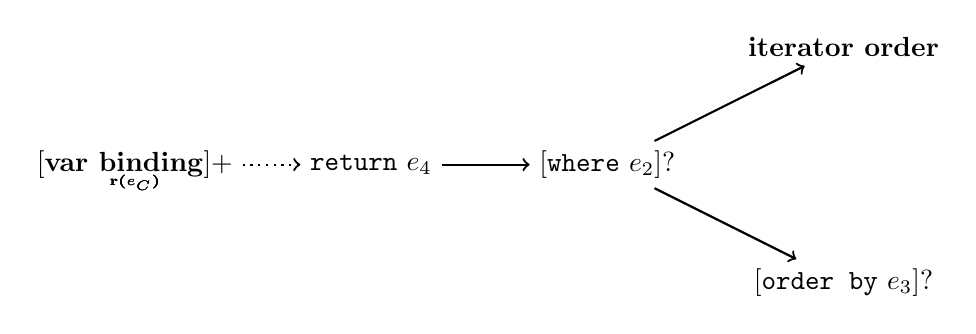
\begin{tikzpicture}

\node (bind) at (0,0) {$[$\textbf{var binding}$]+$};
\node (return) at (3,0) {\texttt{return} $e_{4}$};
\node (where) at (6,0) {$[$\texttt{where} $e_{2}]?$};
\node (itord) at (9,1.5) {\textbf{iterator order}};
\node (ordby) at (9,-1.5) {$[$\texttt{order by} $e_{3}]?$};
\draw [->,dotted,thick] (bind) to (return);
\draw [->,thick] (return) to (where) node[below,midway] {\tiny\textbf{r(}$e_{C}$\textbf{)}};
\draw [->,thick] (where) to (itord) node[below,midway] {\tiny\textbf{r(}$e_{C}$\textbf{)}};
\draw [->,thick] (where) to (ordby) node[below,midway] {\tiny\textbf{r(}$e_{C}$\textbf{)}};
\end{tikzpicture}
\label{fig:trans:TD:flworExecute}
\caption[FLWOR translation order]{Illustration of step-by-step translation of FLWOR.}
\end{figure}



Any possible iteration, ordering og filtering will be handled by other clauses than the \texttt{return} clause.
The \texttt{return} clause will just ship the evaluated version of the \texttt{return} expression forward:
\begin{equation}
\frac{}{\mbox{\texttt{return }}e_{4}}\longmapsto
\mbox{\textbf{r(}}e_{4}\mbox{\textbf{)}}
\label{rule:trans:TD:returnTaint}
\end{equation}


\subsubsection{Iterator Ordering}
The \texttt{return} clause is evaluated once for iteration for each of the iterators of the FLWOR expression. The
results of these evaluations are concatenated to form the result of the FLWOR expression. If the \texttt{return}
expression is not dependent on a iterator, its relational form will not have a representation for each
of the iterators iterations and will have to be tainted.

Because each FLWOR iterator creates a new sequence, renumbering is needed. No expression in a sibling or parent
scope of the iterator $I_{\chi}$ may be dependent on $I_{\chi}$. Thus, $\chi$ is not part of the dependencies
$I_{\chi}.\vartheta$ returned from the iterator, and the corresponding $\chi{numb}$ attribute must be removed. 

For each allready bound iterator variable $\chi$, from right to left, bound in an \texttt{for} clause,
the following translation is applied:
\begin{equation}
\frac{}{\mbox{\textbf{iterator order}}}
\longmapsto
\begin{array}{l}
\mbox{\textsf{numberate(index, [}}\beta\mbox{\textsf{, index], [}}\vartheta\mbox{\textsf{];}} \\ \quad
\mbox{\textbf{t(r(}}e_{C}\mbox{\textbf{), }}\beta\mbox{\textbf{)}}
\end{array}
\label{rule:trans:TD:itOrd}
\end{equation}

Where $\vartheta = e_{C}.\vartheta - \chi$.

From equation \ref{eq:trans:TD:taint} it is clear that a expression allready dependent on any iterator in
$\beta$ will not be re-tainted by these iterators.

The \textsf{numberate} operator will have to partition on the remaining dependencies in $\vartheta$ to seperate
the sequences returned from the iterator for all iterators the result is dependent on, as described in section
\ref{sect:trans:TD:implic}.

\begin{myExample}
Consider the query of figure \ref{fig:trans:TD:dblFor}. Notice the expression in the \texttt{return} clause ($e_1$)
is the same as $e_1$ in example \ref{ex:trans:TD:simpleSeq}.

\begin{figure}[h]
\begin{equation*}
\begin{array}{l}
\mbox{\texttt{for \$a in (10,20),}} \\
\mbox{\texttt{\phantom{abcd}\$b in (50,75)}} \\ 
\mbox{\texttt{return }}\underbrace{\mbox{\texttt{(\$a, "no")}} }_{e_{1}}
\end{array}
\end{equation*}
\caption{Example query with two iterators.}
\label{fig:trans:TD:dblFor}
\end{figure}

Expression $e_{1}$ is not depentant on $I_{\mbox{\texttt{b}}}$, and by rule \ref{rule:trans:TD:itOrd} will be
tainted by this iterator. The result of the tainting is shown in figure \ref{fig:trans:TD:final:taint}. The
expression will however not be tainted by $I_{\mbox{\texttt{a}}}$, as it is allready dependent on this iterator
(ref. equation \ref{eq:trans:TD:taint}).

\begin{figure}[h]
\centering
\subfigure[\textbf{t(r(}$e_{1}$\textbf{), \{}\texttt{b}\textbf{\})}]{
\begin{tabular}{|c|c|c|c|} \hline
$bnumb$ & $anumb$ & $index$ & $value$ \\ \hline
1 & 1 & 1 & 10 \\ \hline
1 & 2 & 1 & 20 \\ \hline
1 & 1 & 2 & \texttt{"no"} \\ \hline
1 & 2 & 2 & \texttt{"no"} \\ \hline
2 & 1 & 1 & 10 \\ \hline
2 & 2 & 1 & 20 \\ \hline
2 & 1 & 2 & \texttt{"no"} \\ \hline
2 & 2 & 2 & \texttt{"no"} \\ \hline
\end{tabular}
\label{fig:trans:TD:final:taint}
}
\qquad
\subfigure[\textbf{r(}$I_{\mbox{\texttt{a}}}$\textbf{)}]{
\begin{tabular}{|c|c|} \hline
$index$ & $value$ \\ \hline
1 & 10 \\ \hline
2 & \texttt{"no"} \\ \hline
3 & 10 \\ \hline
4 & \texttt{"no"} \\ \hline
5 & 20 \\ \hline
6 & \texttt{"no"} \\ \hline
7 & 20 \\ \hline
8 & \texttt{"no"} \\ \hline
\end{tabular}
\label{fig:trans:TD:final:rIa}
}
\caption[Example: resolving simple FLWOR]{Evaluating the query in figure \ref{fig:trans:TD:dblFor} yields the
intermediate result (a) and the final result (b).\label{fig:trans:TD:finalizeExp}}
\end{figure}

With the expression tainted with all possible iterator dependencies of the FLWOR, renumbering is the last
operation required to resolve the query. The \textsf{numberate} operator will sort the tuples first on $anumb$,
then on $bnumb$ and finally $index$ before numbering. As the FLWOR itself does not have any dependencies the
numeration will not be grouped on any attributes. The result of the query is shown in figure
\ref{fig:trans:TD:final:rIa}.
\end{myExample}

\subsubsection{Where Clause}
The W3C describes the FLWOR expression as generating a tuple stream which contains one tuple for each combination
of values bound in the expression\cite{w3c00}. In this view, the optional \texttt{where} clause serves a filter for
these tuples. The expression in the \texttt{where} clause is evaluated once for tuple. If the boolean value of this
expression is $true$, the tuple is retained, if the boolean value is $false$ the tuple is discarded.

The \texttt{where} clause can be evaluated by only selecting the iteration combinations where the \texttt{where}
expression is true. The result of this will be joined with the result of the \texttt{return} clause. If the result
from the \texttt{return} clause and the \texttt{where} expression has no common iterator dependencies, the
equi-join will have to be replaced by a cartesian product, as discussed in \ref{sect:trans:TD:implic}.

\begin{equation}
\frac{}{\mbox{\texttt{where }}e_2}\longmapsto
\begin{array}{l}
\mbox{\textsf{hhjoin([l.}}(e_{C}.\vartheta \cap e_2.\vartheta)\mbox{\textsf{], [r.}}(e_{2}.\vartheta \cap
e_{C}.\vartheta)\mbox{\textsf{], [l.value, }} \vartheta\mbox{\textsf{];}} \\ \quad
\mbox{\textbf{r(}}e_{C}\mbox{\textbf{)\textsf{;}}} \\ \quad
\mbox{\textsf{select(xqBoolean(value);}} \\ \quad \quad
\mbox{\textbf{r(}}e_{2}\mbox{\textbf{)}\textsf{))}}
\end{array}
\label{rule:trans:TD:where}
\end{equation}

Where $\vartheta = e_{C} \cup e_{2}$, and \textbf{r(}$e_{C}$\textbf{)} is the result of the translation done in
the \texttt{return} clause.

\textsf{l.}$(e_{C}.\vartheta \cap e_2.\vartheta)$ is short for
\textsf{l.}$\chi_1$\textsf{numb,\ldots,l.}$\chi_n$\textsf{numb}, where $e_{C}.\vartheta \cap e_2.\vartheta =
\left\{\chi_1,\ldots,\chi_n\right\}$.

By employing the \textsf{select} operator before the joining of the two relations the number of tuples needed to
be read to execute the join will be minimized. Further, as the \textsf{hhjoin} operator allows for declaring which
attributes to be projected, there is no need for a seperate \textsf{project} operator.

\begin{myExample}
Consider the XQuery query of figure \ref{fig:trans:TD:whereQuery}. The evaluation of $e_{1}$ is very similar to
the evaluation of $e_{1}$ of example \ref{ex:trans:TD:simpleSeq}, and the is shown in figure
\ref{fig:trans:TD:where:re1}. The \texttt{where} clause contains a comparison expression, which will be discussed
later. Figure \ref{fig:trans:TD:where:whereE} shows the result relation of the \texttt{where} expression.

\begin{figure}[h]
\centering
\begin{equation*}
\begin{array}{l}
\mbox{\texttt{for \$a in (10,20)}} \\
\mbox{\texttt{where \$a > 15}} \\
\mbox{\texttt{return}} \underbrace{\mbox{\texttt{(\$a, 14)}}}_{e_{1}}
\end{array}
\end{equation*}
\caption{A FLWOR expression with a \texttt{where} clause \label{fig:trans:TD:whereQuery}}
\end{figure}

\begin{figure}[h]
\centering
\subfigure[\textbf{r(}$e_{1}$\textbf{)}]{
\begin{tabular}{|c|c|c|} \hline
$anb$ & $idx$ & $val$ \\ \hline
1 & 1 & 10 \\ \hline
1 & 2 & 14  \\ \hline
2 & 1 & 20 \\ \hline
2 & 2 & 14  \\ \hline
\end{tabular}
\label{fig:trans:TD:where:re1}
}
\qquad
\subfigure[\textbf{r(}\texttt{\$a > 15}\textbf{)}]{
\begin{tabular}{|c|c|c|} \hline
$anb$ & $idx$ & $val$ \\ \hline
1 & 1 & $false$ \\ \hline
2 & 1 & $true$ \\ \hline
\end{tabular}
\label{fig:trans:TD:where:whereE}
}
\qquad
\subfigure[]{
\begin{tabular}{|c|c|c|} \hline
$anb$ & $idx$ & $val$ \\ \hline
2 & 1 & 20 \\ \hline
2 & 2 & 14  \\ \hline
\end{tabular}
\label{fig:trans:TD:where:intr}
}

\caption[Example: Evaluation of where clause]{Applying rule \ref{rule:trans:TD:where} on (a) and (b)
yields (c). Attribute names are shortened. \label{fig:trans:TD:whereClause}}
\end{figure}

During the evaluation of the FLWOR, the tuples in the \texttt{where} expression relation where $value$ ($val$ in
figure) is not $true$ will be removed. The result is a relation with a single tuple where $anumb$ holds the value
$2$. This result is then joined with the $e_1$ relation on $anumb$, as shown in figure
\ref{fig:trans:TD:where:intr}. Rule \ref{rule:trans:TD:itOrd} will have to be applied to complete the
evaluation of the query.
\end{myExample}


\subsubsection{Order By Clause Ordering}

As can be seen in figure \ref{fig:trans:TD:ordEBNF}, an \texttt{Order by} clause may contain several specifications on
how to order and what to order by.
\begin{figure}[h]
\begin{Verbatim}
[38] OrderByClause ::= (("order" "by") | ("stable" "order" "by")) 
                           OrderSpecList
[39] OrderSpecList ::= OrderSpec ("," OrderSpec)*
[40] OrderSpec     ::= ExprSingle OrderModifier
[41] OrderModifier ::= ("ascending" | "descending")? 
                           ("empty" ("greatest" | "least"))? 
                           ("collation" URILiteral)?
\end{Verbatim}
\label{fig:trans:TD:ordEBNF}
\caption[W3C EBNF order by clause specification]{W3C EBNF order by clause specification.}
\end{figure}

At this time, Taiting Dependencies only support a simple form of the clause. Only one \texttt{OrderSpec} is
allowed, where the expression to be sorted on will be referred to as $e_4$ -- conformant to figure
\ref{fig:trans:TD:flworExecute}. No \texttt{OrderModifier}s are allowed, and neither is the \texttt{stable}
option. This will be discussed further in sectin \ref{sect:disc:orderby}.

As with the \texttt{where} clause W3C specify the \texttt{order by} clause as operating on a tuple stream created
by the variable bindings in the FLWOR. The clause causes the stream to be reordered into a new, value-based order.
This means that the iterator dependency attributes ($\chi{numb}$) will no longer decide the composition of the
sequence returned from the FLWOR.

Firstly, to ensure that the result will have a representation for all the iterations (still valid after possible
filtering by \texttt{where} clause) of all the expressions iterators, $e_C$ is tainted with $\beta$. The
\texttt{order by} expression is evaluated and joined with the result of the tainting on their common iterator
dependencies. Lastly, this relation is renumbered according to the order of the values stemming from the
\texttt{order by} expression:

\begin{equation}
\frac{}{\mbox{\texttt{order by }}e_3}\longmapsto
\begin{array}{l}
\mbox{\textsf{project(value = l.value, }}\vartheta\mbox{\textsf{;}}\\ \quad
\mbox{\textsf{numberate(index, [r.value, index], [}}\vartheta\mbox{\textsf{];}} \\ \quad \quad
\mbox{\textsf{hhjoin([l.}}(e_{C}.\vartheta \cap e_2.\vartheta)\mbox{\textsf{], [r.}}(e_{2}.\vartheta \cap
e_{C}.\vartheta)\mbox{\textsf{],}} 
\\ \quad \quad \quad \quad \quad\mbox{\textsf{[l.value, r.value, }} \vartheta\mbox{\textsf{];}} \\ \quad \quad
\quad \mbox{\textbf{t(r(}}e_C\mbox{\textbf{), }}\beta\mbox{\textbf{)}\textsf{;}} \\ \quad \quad \quad
\mbox{\textbf{r(}}e_3\mbox{\textbf{)}\textsf{)))}}
\end{array}
\end{equation}

Where $\vartheta = (e_C.\vartheta \cup e_3.\vartheta)-\beta$, and \textbf{r(}$e_{C}$\textbf{)} is the result of
the translation done in the \texttt{where} clause if present, else the \texttt{return} clause.

As desired, all iterator dependency attributes ($\chi{numb}, \chi \in \beta$) will be projected away by the
\textsf{hhjoin} operator. An additional \textsf{project} operator is used to ensure that the $value$ returned from
the expression is the $value$ attribute of the \texttt{return} expression.

\begin{myExample}
Figure \ref{fig:trans:TD:ordQu} shows a query consisting of a FLWOR expression containing a \texttt{order by} clause.
\begin{figure}[h]
\centering
\begin{tabular}{l}
\texttt{for \$a in (4, 6, 8)} \\
\texttt{order by \$a mod 3}\\
\texttt{return \$a}\\
\end{tabular}
\label{fig:trans:TD:ordQu}
\caption{Example query with order by clause}
\end{figure}

The evaluated \texttt{order by} expression is shown in figure \ref{fig:trans:TD:ord:oExp}. How modulus expressions
are translated will be discussed later. After their evaluation, the relational representation of \texttt{order by}
expression relation and the \texttt{return} clause is joined on their common iterator dependencies,
$I_{\mbox{\texttt{a}}}$. The result of the join is shown in figure \ref{fig:trans:TD:ord:join}. Lastly, this
relation is renumbered sorted on the $r.value$ ($r.val$ in figure) attribute stemming from the \texttt{order by}
expression, as shown in figure \ref{fig:trans:TD:ord:numb}. An additional projection to rename $l.value$ to $value$
is needed to finalise the query.

\begin{figure}[h]
\subfigure[\textbf{r(}\texttt{\$a mod 3}\textbf{)}]{
\begin{tabular}{|c|c|c|} \hline
$idx$ & $anb$ & $val$ \\ \hline
1 & 1 & 1 \\ \hline
1 & 2 & 0 \\ \hline
1 & 3 & 2 \\ \hline
\end{tabular}
\label{fig:trans:TD:ord:oExp}
}
\qquad
\subfigure[]{
\begin{tabular}{|c|c|c|c|} \hline
$l.idx$ & $anb$ & $l.val$ & $r.val$ \\ \hline
1 & 1 & 4 & 1 \\ \hline
1 & 2 & 6 & 0 \\ \hline
1 & 3 & 8 & 2 \\ \hline
\end{tabular}
\label{fig:trans:TD:ord:join}
}
\qquad
\subfigure[]{
\begin{tabular}{|c|c|} \hline
$l.idx$ & $l.val$ \\ \hline
1 & 6 \\ \hline
2 & 4 \\ \hline
3 & 8 \\ \hline
\end{tabular}
\label{fig:trans:TD:ord:numb}
}


\caption{Intermediate results evaluating the query of figure
\ref{fig:trans:TD:ordQu}. (a) shows the evaluated \texttt{order by} expression. (b) shows the \texttt{order by}
expression joined with the \texttt{return} expression. (c) shows the relation in (b) renumbered. Attribute names
are shortened.\label{fig:trans:TD:orderRes}}
\end{figure}


\end{myExample}

\subsection{Arithmetic Expressions}
\label{sect:trans:TD:atrith}
W3C defines the arithmetic expressions as shown in figure \ref{fig:trans:TD:arithEBNF}\cite{w3c00}. Notice how the
specified grammar handles operator precedence. \texttt{UnaryExpr} is a decendant production of \texttt{UnionExpr}.

\begin{figure}[h]
\begin{Verbatim}
[50] AdditiveExpr       ::= MultiplicativeExpr ( ("+" | "-") 
                                MultiplicativeExpr )*
[51] MultiplicativeExpr ::= UnionExpr 
                                ( ("*" | "div" | "idiv" | "mod")
                                UnionExpr )*
[58] UnaryExpr          ::= ("-" | "+")* ValueExpr
\end{Verbatim}
\caption{The arithmetic expressions of XQuery}
\label{fig:trans:TD:arithEBNF}
\end{figure}

The translation of such expressions will have to be separated in binary and unary operators. For the binary
operators the two values to be operated on will have to be in the same relation. To ensure the values to be
operated on are from the same unique iteration (if there is any iterations at all), the relations corresponding to
the two expressions will have to be joined on their common iterator dependencies, as described in section
\ref{sect:trans:TD:implic}. Both the unary and the binary XQuery arithmetic operators accept only singleton
sequences.

\begin{equation}
\frac{}{e_1 \mbox{\texttt{ OP }} e_2}\longmapsto
\begin{array}{l}
\mbox{\textsf{project(index=1,value=FUNC(l.value,r.value),}}\vartheta\mbox{\textsf{;}} \\ \quad
\mbox{\textsf{hhjoin([l.}}(e_1.\vartheta\cap e_2.\vartheta)\mbox{\textsf{], [r.}}(e_2.\vartheta\cap e_1.\vartheta)
\mbox{\textsf{],}} 
\\ \quad \quad \quad \quad\mbox{\textsf{[r.value, l.value, }}\vartheta\mbox{\textsf{];}} \\ \quad \quad
\mbox{\textbf{r(}}e_1\mbox{\textbf{)}} \\ \quad \quad
\mbox{\textbf{r(}}e_2\mbox{\textbf{)}\textsf{))}}
\end{array}
\label{rule:trans:TD:arithmetic}
\end{equation}

Where $\vartheta = e_1.\vartheta \cup e_2.\vartheta$, \texttt{OP} will map to a MQL function replacing
\textsf{FUNC} as shown in table \ref{tab:trans:TD:binOpMap}. The projecting functionality of the
\textsf{hhjoin} operator will in this case remove the $index$ attributes and any possible $documentId$, $scope$
and $pos$ attributes.

\begin{table}[h]
\centering
\begin{tabular}{c|c}
\texttt{OP} & \textsf{FUNC} \\ \hline
\texttt{+} 	& \textsf{sum} \\
\texttt{-} 	& \textsf{subtract} \\
\texttt{*} 	& \textsf{prod} \\
\texttt{div} 	& \textsf{div} \\
\texttt{idiv} 	& \textsf{idiv} \\
\texttt{mod} 	& \textsf{mod} \\
\end{tabular}
\label{tab:trans:TD:binOpMap}
\caption{Mapping XQuery arithmetic operators to MQL functions.}
\end{table}

Considering the unary operators, the \texttt{+} operator will never have any effect, and can therefore be dropped.
The unary \texttt{-} operator will change the sign of the value it is assigned to. This is equal to multiplying
the value with $-1$:
\begin{equation}
\frac{}{\mbox{\texttt{-}}e_1}\longmapsto 
\begin{array}{l}
\mbox{\textsf{project(value = prod(-1, value);}} \\ \quad
\mbox{\textbf{r(}}e_1\mbox{\textbf{)}\textsf{)}}
\end{array}
\label{rule:trans:TD:unaryMin}
\end{equation}

\begin{myExample}
Consider the XQuery query of figure \ref{fig:trans:TD:arithQuery}. Here $e_1$ is an arithmetic expression.

\begin{figure}[h]
\centering
\begin{equation*}
\begin{array}{l}
\mbox{\texttt{for \$a in (1,2) return}} \\ \quad
\mbox{\texttt{for \$b in (3,4) return}} \\ \quad \quad
\underbrace{\mbox{\texttt{\$a + \$b}}}_{e_1}
\end{array}
\end{equation*}
\caption{Example query containting a arithmetic expression.}
\label{fig:trans:TD:arithQuery}
\end{figure}

Both \texttt{\$a} and \texttt{\$b} is translated to simple two-tuple relations by rules
\ref{rule:trans:TD:forbind} and \ref{rule:trans:TD:varRef}. As the two expressions do not have any iterator
dependencies the \texttt{hhjoin} operator of rule \ref{rule:trans:TD:arithmetic} will be treated as a cartesian
product (ref. \ref{sect:trans:TD:implic}). The cross product of the two relations are shown in figure
\ref{fig:trans:TD:aritJoin}. Lastly, the \texttt{project} operator is employed to calculate the sum for each
iteration, the result of which is shown in figure \ref{fig:trans:TD:aritEnd}.

\begin{figure}[h]
\centering
\subfigure[]{
\begin{tabular}{|c|c|c|c|}\hline
$anb$ & $bnb$ & $l.val$ & $r.val$ \\ \hline
1 & 1 & 1 & 3 \\ \hline
2 & 1 & 2 & 3 \\ \hline
1 & 2 & 1 & 4 \\ \hline
2 & 2 & 2 & 4 \\ \hline
\end{tabular}
\label{fig:trans:TD:aritJoin}
}
\qquad
\subfigure[\textbf{r(}$e_1$\textbf{)}]{
\begin{tabular}{|c|c|c|c|}\hline
$idx$ & $anb$ & $bnb$ & $val$ \\ \hline
1 & 1 & 1 & 4 \\ \hline
1 & 2 & 1 & 5 \\ \hline
1 & 1 & 2 & 5 \\ \hline
1 & 2 & 2 & 6 \\ \hline
\end{tabular}
\label{fig:trans:TD:aritEnd}
}
\caption[Results of evaluating expression $e_1$ of figure \ref{fig:trans:TD:arithQuery}.]{Results of evaluating
expression $e_1$ of figure \ref{fig:trans:TD:arithQuery}. (a) shows the result of the cross product. (b) is the
fully evaluated $e_1$. Attribute names are shortened. \label{fig:trans:TD:arithRes}}
\end{figure}

\end{myExample}

\subsection{Logical Expressions}
\label{sect:trans:TD:logical}
An XQuery logical expression is either an \texttt{and} expression or an \texttt{or} expression. If a logical
expression does not raise an error, its value is always one of the boolean values $true$ or $false$.

A logical expression is translated in a matter very similar to the arithmetic expressions. The XQuery logical
operators does however operate on the effective boolean value (see section \ref{sect:theory:xquery:basics}) rather
than the direct value. Rule \ref{rule:trans:TD:arithmetic} is valid for logical expressions, and the mapping
between the XQuery operators and the MQL functions are shown in table JEJEJEJE. As the operators require effective
boolean values, the $value$ fields will have to be run through the \textsf{xqBoolean()} function. E.g. the
following will be a part of the parameters of the \textsf{project} operator of a translated \texttt{or} expression:
\textsf{\ldots value = or(xqBoolean(l.value),xqBoolean(r.value))\ldots}.

\begin{table}[h]
\centering
\begin{tabular}{c|c}
\texttt{OP} & \textsf{FUNC} \\ \hline
\texttt{or} & \textsf{or} \\
\texttt{and} & \textsf{and} \\
\end{tabular}
\label{tab:trans:TD:logMap}
\caption{Mapping XQuery boolean operators to MQL functions}
\end{table}

For logical expressions, $e_1$\texttt{ logOp }$e_2$, $e_1$ and $e_2$ and their possible subexpressions will have
to be translated in the logical context $\Lambda$.

\subsection{Comparative Expressions}
\label{sect:trans:TD:compArit}
Comparison expressions allow two values to be compared. XQuery provides three kinds of comparison expressions,
called value comparisons, general comparisons, and node comparisons. The comparison operators as specified by W3C
are shown in figure \ref{fig:trans:TD:compEBNF}. The Tainting Dependency method does at this time not support node
comparison, as will be discussed in section \ref{sect:disc:notSupported}.

\begin{figure}[h]
\begin{Verbatim}
[61] ValueComp   ::= "eq" | "ne" | "lt" | "le" | "gt" | "ge"
[60] GeneralComp ::= "=" | "!=" | "<" | "<=" | ">" | ">="
[62] NodeComp    ::= "is" | "<<" | ">>"
\end{Verbatim}
\caption{The comparison operators of XQuery}
\label{fig:trans:TD:compEBNF}
\end{figure}

Value comparisons are used for comparing two single values. With the same premises and restrictions the rule for
translating arithmetic expressions (rule \ref{rule:trans:TD:arithmetic}) can be used to translate such comparison
expressions. The mapping between the XQuery value comparators and MQL functions can be seen in table
\ref{tab:trans:TD:valueComp}.

\begin{table}[h]
\centering
\begin{tabular}{c|c}
\texttt{OP} & \textsf{FUNC} \\ \hline
\texttt{eq} & \textsf{eq} \\
\texttt{ne} & \textsf{neq} \\
\texttt{lt} & \textsf{lt} \\
\texttt{le} & \textsf{leq} \\
\texttt{gt} & \textsf{gt} \\
\texttt{ge} & \textsf{geq} \\
\end{tabular}
\label{tab:trans:TD:valueComp}
\caption{Mapping XQuery value comparators to MQL functions}
\end{table}

General comparisons are existentially quantified comparisons that may be applied to sequences of any length. If
employing a general comparator on any pair of items consisting of one from each of the sequences yields $true$,
the comparison expression yields true. As an example, all the comparison expressions of figure
\ref{fig:trans:TD:genCompEx} evaluates to $true$.

\begin{figure}[h]
\centering
\begin{tabular}{l}
\texttt{(1, 2) = (2, 3)} \\
\texttt{(1, 2) != (2, 3)} \\
\texttt{(1, 200) < (10, 20)} \\
\texttt{(1, 200) > (10, 20)} \\
\end{tabular}
\label{fig:trans:TD:genCompEx}
\caption[Example general comparisons]{Example general comparisons: all expressions evaluate to $true$}
\end{figure}

The big difference between general and value comparisons is that the first must accomodate for sequences. This is
solved by grouping expressions' iterator dependencies, meaning that each group will contain the sequence of one
unique iteration. By defining $true$ as having a larger value than $false$, the \textsf{max()} aggregator will
identify the groups with \emph{at least} one $true$ value.

As with the arithmetic expressions, the relational representation of the two operands is joined on their common
dependencies to ensure that both values are from the same iteration.

\begin{equation}
\frac{}{e_1\mbox{\texttt{ OP }}e_2}\longmapsto
\begin{array}{l}
\mbox{\textsf{project(index = 1, value=max, }}\vartheta \textsf{;} \\ \quad
\mbox{\textsf{group((}}\vartheta\mbox{\textsf{), max(value);}} \\ \quad \quad
\mbox{\textsf{project(value=FUNC(r.value,l.value),}}\vartheta\mbox{\textsf{;}} \\ \quad \quad \quad
\mbox{\textsf{hhjoin([l.}}(e_1.\vartheta\cap e_2.\vartheta)\mbox{\textsf{], [r.}}(e_2.\vartheta\cap e_1.\vartheta)
\mbox{\textsf{],}} 
\\ \quad \quad \quad \quad \quad \quad\mbox{\textsf{[l.value, r.value, }}\vartheta\mbox{\textsf{];}} \\ \quad \quad
\quad \quad \quad \mbox{\textbf{r(}}e_1\mbox{\textbf{)}} \\ \quad \quad \quad \quad \quad
\mbox{\textbf{r(}}e_2\mbox{\textbf{)}\textsf{))))}}
\end{array}
\label{rule:trans:TD:comparative}
\end{equation}

Where $\vartheta = e_1.\vartheta \cup e_2.\vartheta$. \texttt{OP} wil map to a MQL function replacing
\textsf{FUNC} as shown in table \ref{tab:trans:TD:genCompMap}. 

The result of a general comparison is always a singleton sequence, thus it is safe to project in an $index$
attribute with the value $1$. The $index$ and possible $documentId$, $scope$ and $pos$ attributes are left out of
the project list of the \textsf{hhjoin} operator.

\begin{table}[h]
\centering
\begin{tabular}{c|c}
\texttt{OP} & \textsf{FUNC} \\ \hline
\texttt{=} & \textsf{eq} \\
\texttt{!=} & \textsf{neq} \\
\texttt{<} & \textsf{lt} \\
\texttt{<=} & \textsf{leq} \\
\texttt{>} & \textsf{gt} \\
\texttt{>=} & \textsf{geq} \\
\end{tabular}
\label{tab:trans:TD:genCompMap}
\caption{Mapping XQuery general comparators to MQL functions.}
\end{table}

\begin{myExample}
Figure \ref{fig:trans:TD:genCompQu} shows a simple XQuery query with a general comparison expression, $e_1$.
\begin{figure}[h]
\centering
\begin{equation*}
\begin{array}{l}
\mbox{\texttt{for \$a in (10, 20) return}} \\ \quad
\underbrace{\mbox{\texttt{\$a > (5, 15)}}}_{e_1}
\end{array}
\end{equation*}
\caption{Example query with a general comparison expression \label{fig:trans:TD:genCompQu}}
\end{figure}
 
Because the operands of the \texttt{>} operator have no common iterator dependencies, the cartesian product of the
two relations are calculated, as seen in figure \ref{fig:trans:TD:gen:join}. After the inner \textsf{project}
operator is employed, the result will be as in figure \ref{fig:trans:TD:gen:projGr}. The double line illustrates
the grouping on $anumb$ ($anb$ in the figure). The maximum value of $value$ for each group is calculated and the
attributes are renamed, which gives the relation of figure \ref{fig:trans:TD:gen:end}.

\begin{figure}[h]
\centering
\subfigure[]{
\begin{tabular}{|c|c|c|} \hline
$anb$ & $l.val$ & $r.val$ \\ \hline
1 & 10 & 5 \\ \hline
1 & 10 & 15 \\ \hline
2 & 20 & 5 \\ \hline
2 & 20 & 15 \\ \hline
\end{tabular}
\label{fig:trans:TD:gen:join}
}
\qquad
\subfigure[]{
\begin{tabular}{|c|c|} \hline
$anb$ & $val$ \\ \hline
1 & $true$ \\ \hline
1 & $false$ \\ \hline \hline
2 & $true$ \\ \hline
2 & $true$ \\ \hline
\end{tabular}
\label{fig:trans:TD:gen:projGr}
}
\qquad
\subfigure[\textbf{r(}$e_1$\textbf{)}]{
\begin{tabular}{|c|c|c|} \hline
$idx$ & $anb$ & $val$ \\ \hline
1 & 1 & $true$ \\ \hline
1 & 2 & $true$ \\ \hline
\end{tabular}
\label{fig:trans:TD:gen:end}
}
\caption[Results of evaluating $e_1$ in figure \ref{fig:trans:TD:genCompQu}]{Results of evaluating expression $e_1$
in figure \ref{fig:trans:TD:genCompQu}. (a) The relations of the operands joined. (b) Each combination of the
sequences evaluated. Double line illustrates grouping. (c) The final result. Attribute names are shortened.
\label{fig:trans:TD:genCompRes}}
\end{figure}
 
\end{myExample}


\subsection{Path Expressions}
\label{sect:trans:TD:pathExprs}
\begin{itemize}
  \item axes
  \item samling av child axes /a/b/c/d -> ikke e1/e2
  \item i logical context -> outer join
\end{itemize}

\subsection{Predicates}
\label{sect:trans:TD:predicates}
\begin{itemize}
  \item isNumber() ifThenElse xqBoolean()
  \item contextnode p\aa~boks\ldots trengs dette alltid? Strengt tatt.. veldig vanskelig \aa~vite n\aa r man
  garantert ikke trenger den iallefall\ldots
\end{itemize}

\subsection{Conditional Expressions}
\label{sect:trans:TD:ifThenElse}
\begin{itemize}
  \item if(e1) then else
  \item e1 er i logical context..
\end{itemize}

\subsection{Full Text Expressions}
\label{sect:trans:TD:fulltext}
\begin{itemize}
  \item lookup.. passe p\aa~ contextnode
\end{itemize}

\subsection{other Th1ngz:}
\begin{itemize}
  \item node comparisons\ldots\ldots tviler p\aa~at vi f\aa r til dette glatt\ldots
  \item constructors\ldots element, CDATA, attribute etc etc
\end{itemize}


\subsection{Optimisations}
\label{sect:trans:TD:optimisations}
\begin{itemize}
  \item sekvenser:
	  \begin{itemize}
	    \item suprIndx kan doppes n\aa r bare singelton
	    \item singeltons trenger ikke index
      \end{itemize} 
  \item Litterals: 
		\begin{itemize}
          \item implies that any sequence of
				explicitly stated items will first have to be made as one-tuple relations and
				then spliced together. As the \textsf{make} operator supports multiple items, a
					better solution would be to collect all items in one MQL operator. Further, if
					the item is part of a singleton sequence, there is no need for a representation
					in form of an relation, as the item could be made part of the parameters of an
					operator (e.g. $\alpha$ \texttt{> 1} $\Longrightarrow$
					\textsf{select(gt(value, 1) $\alpha$)}).   
        \end{itemize}
  \item FLWOR:
  	\begin{itemize}
        \item  kan bli -> project , ved singelton return
      \end{itemize}   
  \item Arithmetic /comp / logical
	\begin{itemize}
      \item multiple +- kan bli dyttet sammen\ldots oddetall - = -, partal = drit i det.
      \item singleton inn i and/or -> slippe select
    \end{itemize}
  \item             
\end{itemize}